%% -*- coding: utf-8 -*-
\documentclass[12pt,a4paper]{scrartcl} 
\usepackage[utf8]{inputenc}
\usepackage[english,russian]{babel}
\usepackage{indentfirst}
\usepackage{misccorr}
\usepackage{graphicx}
\usepackage{amsmath}
\usepackage{float}

\usepackage{xcolor}
\usepackage{hyperref}
\hypersetup{colorlinks,
  pdftitle={The title of your document},
  pdfauthor={Your name},
  allcolors=[RGB]{000 000 000}}

\begin{document}
\begin{titlepage}
  \begin{center}

    Санкт-Петербургский политехнический университет Петра Великого

    \vspace{0.25cm}
    
    Институт прикладной математики и механики
    
    Кафедра «Прикладная математика»
    \vfill

	\vspace{0.25cm}
	    Отчёт\\
	по лабораторной работе №6\\
	по дисциплине\\
	«Математическая статистика»

  \bigskip

\end{center}
\vfill

\newlength{\ML}
\settowidth{\ML}{«\underline{\hspace{0.7cm}}» \underline{\hspace{2cm}}}
\hfill\begin{minipage}{0.4\textwidth}
  Выполнил студент\\ В.\,А.~Рыженко\\
\end{minipage}%
\bigskip

\hfill\begin{minipage}{0.4\textwidth}
  Проверил:\\
к.ф.-м.н., доцент\\
Баженов Александр Николаевич\\
\end{minipage}%
\vfill

\begin{center}
  Санкт-Петербург, 2020 г.
\end{center}
\end{titlepage}

\tableofcontents
\listoffigures
\newpage

\section{Постановка задачи}
 
Найти оценки коэффициентов линейной регрессии $y_{i} = a + bx_{i} + e_{i}$, используя 20 точек на отрезке [-1.8; 2] с равномерным шагом равным 0.2. Ошибку $e_{i}$ считать нормально распределённой с параметрами (0, 1). В качестве эталонной зависимости взять $y_{i} = 2 + 2x_{i} + e_{i}$. При построении оценок коэффициентов использовать два критерия: критерий наименьших квадратов и критерий наименьших модулей. Проделать то же самое для выборки, у которой в значения $y_{1}$ и $y_{20}$ вносятся возмущения 10 и -10.

\section{Теория}

\subsection{Простая линейная регрессия}

\subsection{Двумерное нормальное распределение}
    Регрессионную модель описания данных называют простой линейной регрессией, если
	\begin{equation}
	    y_{i} = \beta_{0} + \beta_{1}x_{i} + \epsilon_{i},  i = 1..n
	    \label{y_i}
	\end{equation}
	где $x_{1},...,x_{n}$ — заданные числа (значения фактора); $y_{1},...,y_{n}$ — наблюдаемые значения отклика; $\epsilon_{1},...,\epsilon_{n}$ — независимые, нормально распределённые N(0,$\sigma$) с нулевым математическим ожиданием и одинаковой (неизвестной) дисперсией случайные величины (ненаблюдаемые); $\beta_{0}$, $\beta_{1}$ — неизвестные параметры, подлежащие оцениванию.
    В модели (\ref{y_i}) отклик y зависит зависит от одного фактора x, и весь разброс экспериментальных точек объясняется только погрешностями наблюдений (результатов измерений) отклика y. Погрешности результатов измерений x в этой модели полагают существенно меньшими погрешностей результатов измерений y, так что ими можно пренебречь [1, с. 507].


	
	\subsubsection{Метод наименьших квадратов}
	При оценивании параметров регрессионной модели используют различные методы. Один из наиболее распрстранённых подходов заключается в следующем: вводится мера (критерий) рассогласования отклика и регрессионной функции, и оценки параметров регрессии определяются так, чтобы сделать это рассогласование наименьшим. Достаточно простые расчётные формулы для оценок получают при выборе критерия в виде суммы квадратов отклонений значений отклика от значений регрессионной функции (сумма квадратов остатков):
	\begin{equation}
	    Q(\beta_{0}, \beta_{1}) = \sum_{i=1}^{n}{\epsilon_{i}^{2}} = 
	    \sum_{i=1}^{n}{(y_{i} - \beta_{0} - \beta_{1}x_{i})^{2}}\rightarrow \min_{\beta_{0}, \beta_{1}}
	    \label{Q_beta}
	\end{equation}
	Задача минимизации квадратичного критерия (\ref{Q_beta}) носит название задачи метода наименьших квадратов (МНК), а оценки $\hat{\beta_{0}}, \hat{\beta_{1}}$ параметров $\beta_{0}, \beta_{1}$, реализующие минимум критерия (\ref{Q_beta}), называют МНК-оценками [1, с. 508]. 

	\subsubsection{Расчётные формулы для МНК-оценок}
	МНК-оценки параметров $\hat{\beta_{0}}, \hat{\beta_{1}}$ находятся из условия обращения функции $Q(\beta_{0}, \beta_{1})$ в минимум. 
	\newline
	Для нахождения МНК-оценок $\hat{\beta_{0}}, \hat{\beta_{1}}$ выпишем необходимые условия экстремума
	\begin{equation}
	   \begin{cases}
         & \frac{\partial Q}{\partial \beta_{0}}  = 
         -2\sum_{i=1}^{n}{(y_{i} - \beta_{0} - \beta_{1}x_{i})} = 0\\ 
         & \frac{\partial Q}{\partial \beta_{1}}  = 
         -2\sum_{i=1}^{n}{(y_{i} - \beta_{0} - \beta_{1}x_{i})x_{i}} = 0 
       \end{cases}
       \label{sys_min}
	\end{equation}
	Далее для упрощения записи сумм будем опускать индекс суммирования. Из системы (\ref{sys_min}) получим:
	\begin{equation}
	   \begin{cases}
         & n\hat{\beta_{0}} + \hat{\beta_{1}}\sum_{}{}{x_{i}} = 
         \sum_{}{}{y_{i}}\\ 
        & \hat{\beta_{0}}\sum_{}{}{x_{i}} + \hat{\beta_{1}}\sum_{}{}{x_{i}^{2}} = \sum_{}{}{x_{i}y_{i}}
       \end{cases}
       \label{sys_2}
	\end{equation}
	Разделим оба уравнения на n:
	\begin{equation}
	   \begin{cases}
         & \hat{\beta_{0}} + \hat{\beta_{1}}(\frac{1}{n}\sum_{}{}{x_{i}}) = 
         \frac{1}{n}\sum_{}{}{y_{i}}\\ 
        & \hat{\beta_{0}}(\frac{1}{n}\sum_{}{}{x_{i}}) + \hat{\beta_{1}}(\frac{1}{n}\sum_{}{}{x_{i}^{2}}) = \frac{1}{n}\sum_{}{}{x_{i}y_{i}}
       \end{cases}
       \label{sys_3}
	\end{equation}
	и, используя известные статистические обозначения для выборочных первых и вторых начальных моментов
	\begin{equation}
	    \bar{x} = \frac{1}{n}\sum_{}{}{x_{i}}, \bar{y} = \frac{1}{n}\sum_{}{}{y_{i}}, \bar{x^{2}} = \frac{1}{n}\sum_{}{}{x_{i}^{2}}, \bar{xy} = \frac{1}{n}\sum_{}{}{x_{i}y_{i}}, 
	\end{equation}
	получим
		\begin{equation}
	   \begin{cases}
         & \hat{\beta_{0}} + \hat{\beta_{1}}\bar{x} = 
         \bar{y}\\ 
        & \hat{\beta_{0}}\bar{x} + \hat{\beta_{1}}\bar{x^{2}} = \bar{xy},
       \end{cases}
       \label{sys_fin}
	\end{equation}
	откуда МНК-оценку $\hat{\beta_{1}}$ наклона прямой регрессии находим по формуле Крамера
	\begin{equation}
	    \hat{\beta_{1}} = \frac{\bar{xy} - \bar{x} \cdot \bar{y}}{\bar{x^{2}} - (\bar{x})^{2}}
	    \label{beta_1_new}
	\end{equation}
	a МНК-оценку $\hat{\beta_{0}}$  определяем непосредственно из первого уравнения системы (\ref{sys_fin}):
	\begin{equation}
	    \hat{\beta_{0}} = \bar{y} - \bar{x}\hat{\beta_{1}}
	    \label{beta_0_new}
	\end{equation}
	Заметим, что определитель системы (\ref{sys_fin}):
	\begin{equation}
	    \bar{x^{2}} - (\bar{x})^{2} = \frac{1}{n}\sum_{}{}{(x_{i} - \bar{x})^{2}} = s_{x}^{2} > 0, 
	\end{equation}
	если среди значений $x_{1},...,x_{n}$ есть различные, что и будем предполагать.
	\newline
	Доказательство минимальности функции $Q(\beta_{0}, \beta_{1})$ в стационарной точке проведём с помощью известного достаточного признака экстремума функции двух переменных. Имеем:
	\begin{equation}
	    \frac{\partial ^{2} Q}{\partial \beta_{0}^{2}} = 2n, 
        \frac{\partial ^{2} Q}{\partial \beta_{1}^{2}} = 2\sum_{}{}{x_{i}^{2}} = 2n\bar{x^{2}}, 
        \frac{\partial ^{2} Q}{\partial \beta_{1} \partial \beta_{0}} = 2\sum_{}{}{x_{i}} = 2n\bar{x}
        \label{frac_eq}
	\end{equation}
	\begin{equation}
	    \bigtriangleup = \frac{\partial^{2}Q}{\partial \beta_{0}^{2}} \cdot \frac{\partial^{2}Q}{\partial \beta_{1}^{2}} - (\frac{\partial^{2}Q}{\partial \beta_{1} \partial \beta_{0}})^{2} = 
	    4n^{2}\bar{x^{2}} - 4n^2(\bar{x})^{2} = 
	    4n^{2}\left[\bar{x^{2}} - (\bar{x})^{2}\right] = 4n^{2}\left[ \frac{1}{n}\sum{}_{}{(x_{i} - \bar{x})}\right] = 4n^{2}s_{x}^{2} > 0.
	    \label{det_sys}
	\end{equation}
	Этот результат вместе с условием $\frac{\partial^{2}Q}{\partial \beta_{0}^{2}} = 2n > 0$ означает, что в стационарной точке функция Q имеет минимум.

    \subsection{Робастные оценки коэффициентов линейной регрессии}
    Робастность оценок коэффициентов линейной регрессии (т.е. их устойчивость по отношению к наличию в данных редких, но больших по величине выбросов) может быть обеспечена различными способами. Одним из них является использование метода наименьших модулей вместо метода наименьших квадратов:
    \begin{equation}
	    \sum_{i=1}^{n}{|y_{i} - \beta_{0} - \beta_{1}x_{i}|}\rightarrow \min_{\beta_{0}, \beta_{1}}
	    \label{min_abs}
	\end{equation}
    Напомним, что использование метода наименьших модулей в задаче оценивания параметра сдвига распределений приводит к оценке в виде выборочной медианы, обладающей робастными свойствами. В отличие от этого случая и от задач метода наименьших квадратов, на практике задача (\ref{min_abs}) решается численно. Соответствующие процедуры представлены в некоторых современных пакетах программ по статистическому анализу.
    \newline
    Здесь мы рассмотрим простейшую в вычистлительном отношении робастную альтернативу оценкам коэффициентов линейной регрессии по МНК. Для этого сначала запишем выражения для оценок (\ref{beta_0_new}) и (\ref{beta_1_new}) в другом виде: 
    \begin{equation}
        \hat{\beta_{1}} = \frac{\bar{xy} - \bar{x} \cdot \bar{y}}{\bar{x^{2}} - (\bar{x})^{2}} = \frac{k_{xy}}{s_{x}^{2}} = \frac{k_{xy}}{s_{x}s_{y}} \cdot \frac{s_{y}}{s_{x}} = r_{xy}\frac{s_{y}}{s_{x}},\\
        \hat{\beta_{0}} = \bar{y} - \bar{x}\hat{\beta_{1}}
        \label{new_coef_abs}
    \end{equation}
    В формулах (\ref{new_coef_abs}) заменим выборочные средние $\bar{x}$ и $\bar{y}$ соответственно на робастные выборочные медианы med x и med y, среднеквадратические отклонения $s_{x}$ и $s_{y}$ на робастные нормированные интерквартильные широты $q^{*}_{x}$ и $q^{*}_{y}$, выборочный коэффициент корреляции $r_{xy}$ — на знаковый коэффициент корреляции $r_{Q}$: 
    \begin{equation}
        \hat{\beta_{1}}_{R} = r_{Q}\frac{q^{*}_{y}}{q^{*}_{x}},
        \label{b_1R}
    \end{equation}
    \begin{equation}
        \hat{\beta_{0}}_{R} = med y - \hat{\beta_{1}}_{R} med x,
        \label{b_0R}
    \end{equation}
    \begin{equation}
        r_{Q} = \frac{1}{n}\sum_{i=1}^{n}{sgn(x_{i} - med x)sgn(y_{i} - med y)},
        \label{r_Q}
    \end{equation}
    \begin{multline}
        \\\\
        q^{*}_{y} = \frac{y_{(j)} -y_{(l)}}{k_{q}(n)}, 
        q^{*}_{x} = \frac{x_{(j)} - x_{(l)}}{k_{q}(n)}, \\ 
        \begin{cases}
             & [\frac{n}{4}] + 1 \text{ при } \frac{n}{4} \text{ дробном, } \\ 
             & \frac{n}{4} \text{ при } \frac{n}{4} \text{ целом. }
        \end{cases}\\
        j = n - l + 1\\
        sgn(z) = \begin{cases}
                    & 1 \text{ при } z > 0 \\ 
                    & 0 \text{ при } z = 0 \\
                    & -1 \text{ при } z < 0
                 \end{cases}\\
        \label{q*}        
    \end{multline}
    Уравнение регрессии здесь имеет вид 
    \begin{equation}
        y = \hat{\beta_{0}}_{R} +  \hat{\beta_{1}}_{R}x
        \label{y}
    \end{equation}
    Статистики выборочной медианы и интерквартильной широты обладают робастными свойствами в силу того, что основаны на центральных порядковых статистиках, малочувствительных к большим по величине выбросам в данных. Статистика выборочного знакового коэффициента корреляции робастна, так как знаковая функция sgn z чувствительна не к величине аргумента, а только к его знаку. Отсюда оценка прямой регрессии (\ref{y}) обладает очевидными робастными свойствами устойчивости к выбросам по координате y, но она довольно груба

 \subsection{Оценка качества}
Проводить оценку качества работы метод будем проводить при помощи метода наименьших квадратов \ref{min_abs}

\section {Реализация}
Лабораторная работа выполнена с помощью встроенных средств языка программирования Python в среде разработки Visual Code. Исходный код лабораторной работы приведён в приложении.
 
\section{Результаты}
\subsection{Оценки коэффициентов линейной регрессии}
	\subsubsection{Выборка без возмущений}
	\begin{itemize}
	    \item{Критерий наименьших квадратов:}
	    $\hat{a}\approx 2.36$, $\hat{b}\approx 2.06,$ quality $ \approx  12.63 $
	    \item{Критерий наименьших модулей:}
	     $\hat{a}\approx$ 2.65, $\hat{b}\approx 2.14,$ quality $\approx  13.79$
	\end{itemize}
	\begin{figure}[H]
	    \centering
	    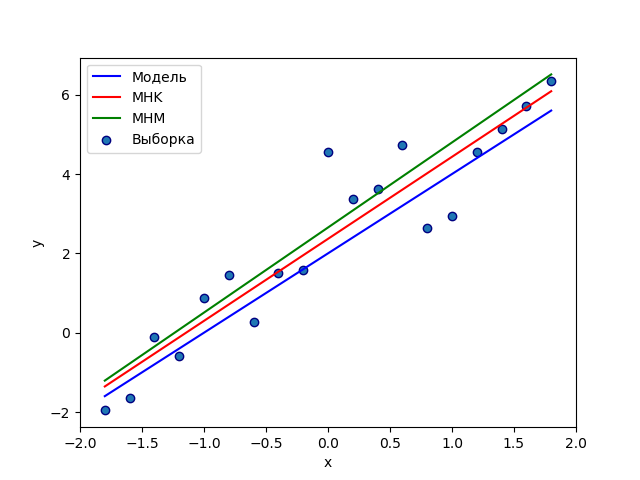
\includegraphics[width = 10cm, height = 8cm]{notperturbation_lab6.png}
	    \caption{Выборка без возмущений}
	    \label{w/o_dist}
	\end{figure}
	
	\subsubsection{Выборка с возмущениями}
	\begin{itemize}
	    \item{Критерий наименьших квадратов:}
	    $\hat{a}\approx 2.36$, $\hat{b}\approx 0.48,$ quality $\approx  38.23$
	    \item{Критерий наименьших модулей:}
	     $\hat{a}\approx 2.65$, $\hat{b}\approx 1.69,$ quality $\approx  30.76$
	\end{itemize}
	\begin{figure}[H]
	    \centering
	    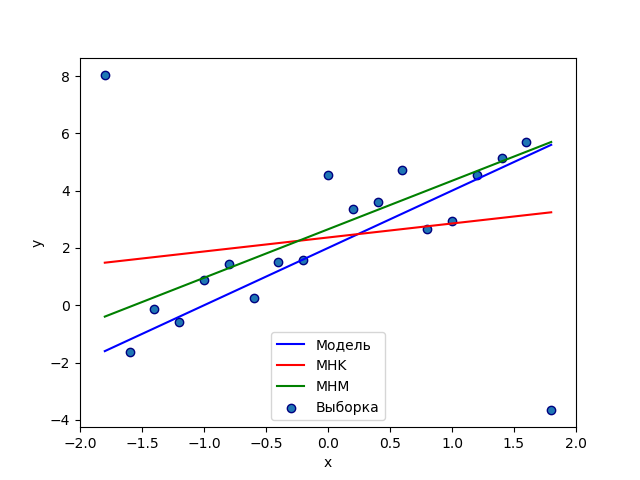
\includegraphics[width = 10cm, height = 8cm]{perturbation_lab6.png}
	    \caption{Выборка с возмущениями}
	    \label{w/o_dist}
	\end{figure}

\section{Обсуждение}
\begin{itemize}
\itemКритерий наименьших квадратов точнее оценивает коэффициенты линейной регрессии на выборке без возмущений. 
\item
Для выборки с возмущениями результат получается точнее при оценке критерием наименьших модулей.
\item
Таким образом, критерий наименьших модулей устойчив к редким выбросам, в отличие от критерия наименьших квадратов.
\end{itemize}
\section{Приложения}
Репозиторий на GitHub с релизацией: \href{https://github.com/WiillyWonka/MatStat}{github.com}.

\begin{thebibliography}{99}
		 \bibitem{max}   Вероятностные разделы математики. Учебник для бакалавров технических направлений.//Под ред. Максимова Ю.Д. — Спб.: «Иван Федоров», 2001. — 592 c., илл.
		 \bibitem{regr}  Вентцель Е.С. Теория вероятностей: Учеб. для вузов. — 6-е изд. стер. — М.: Высш. шк., 1999.— 576 c.
\end{thebibliography}

\end{document}